
\documentclass{article} % For LaTeX2e
\usepackage{iclr2025_conference,times,graphicx}

% Optional math commands from https://github.com/goodfeli/dlbook_notation.
%%%%% NEW MATH DEFINITIONS %%%%%

\usepackage{amsmath,amsfonts,bm}

% Mark sections of captions for referring to divisions of figures
\newcommand{\figleft}{{\em (Left)}}
\newcommand{\figcenter}{{\em (Center)}}
\newcommand{\figright}{{\em (Right)}}
\newcommand{\figtop}{{\em (Top)}}
\newcommand{\figbottom}{{\em (Bottom)}}
\newcommand{\captiona}{{\em (a)}}
\newcommand{\captionb}{{\em (b)}}
\newcommand{\captionc}{{\em (c)}}
\newcommand{\captiond}{{\em (d)}}

% Highlight a newly defined term
\newcommand{\newterm}[1]{{\bf #1}}


% Figure reference, lower-case.
\def\figref#1{figure~\ref{#1}}
% Figure reference, capital. For start of sentence
\def\Figref#1{Figure~\ref{#1}}
\def\twofigref#1#2{figures \ref{#1} and \ref{#2}}
\def\quadfigref#1#2#3#4{figures \ref{#1}, \ref{#2}, \ref{#3} and \ref{#4}}
% Section reference, lower-case.
\def\secref#1{section~\ref{#1}}
% Section reference, capital.
\def\Secref#1{Section~\ref{#1}}
% Reference to two sections.
\def\twosecrefs#1#2{sections \ref{#1} and \ref{#2}}
% Reference to three sections.
\def\secrefs#1#2#3{sections \ref{#1}, \ref{#2} and \ref{#3}}
% Reference to an equation, lower-case.
\def\eqref#1{equation~\ref{#1}}
% Reference to an equation, upper case
\def\Eqref#1{Equation~\ref{#1}}
% A raw reference to an equation---avoid using if possible
\def\plaineqref#1{\ref{#1}}
% Reference to a chapter, lower-case.
\def\chapref#1{chapter~\ref{#1}}
% Reference to an equation, upper case.
\def\Chapref#1{Chapter~\ref{#1}}
% Reference to a range of chapters
\def\rangechapref#1#2{chapters\ref{#1}--\ref{#2}}
% Reference to an algorithm, lower-case.
\def\algref#1{algorithm~\ref{#1}}
% Reference to an algorithm, upper case.
\def\Algref#1{Algorithm~\ref{#1}}
\def\twoalgref#1#2{algorithms \ref{#1} and \ref{#2}}
\def\Twoalgref#1#2{Algorithms \ref{#1} and \ref{#2}}
% Reference to a part, lower case
\def\partref#1{part~\ref{#1}}
% Reference to a part, upper case
\def\Partref#1{Part~\ref{#1}}
\def\twopartref#1#2{parts \ref{#1} and \ref{#2}}

\def\ceil#1{\lceil #1 \rceil}
\def\floor#1{\lfloor #1 \rfloor}
\def\1{\bm{1}}
\newcommand{\train}{\mathcal{D}}
\newcommand{\valid}{\mathcal{D_{\mathrm{valid}}}}
\newcommand{\test}{\mathcal{D_{\mathrm{test}}}}

\def\eps{{\epsilon}}


% Random variables
\def\reta{{\textnormal{$\eta$}}}
\def\ra{{\textnormal{a}}}
\def\rb{{\textnormal{b}}}
\def\rc{{\textnormal{c}}}
\def\rd{{\textnormal{d}}}
\def\re{{\textnormal{e}}}
\def\rf{{\textnormal{f}}}
\def\rg{{\textnormal{g}}}
\def\rh{{\textnormal{h}}}
\def\ri{{\textnormal{i}}}
\def\rj{{\textnormal{j}}}
\def\rk{{\textnormal{k}}}
\def\rl{{\textnormal{l}}}
% rm is already a command, just don't name any random variables m
\def\rn{{\textnormal{n}}}
\def\ro{{\textnormal{o}}}
\def\rp{{\textnormal{p}}}
\def\rq{{\textnormal{q}}}
\def\rr{{\textnormal{r}}}
\def\rs{{\textnormal{s}}}
\def\rt{{\textnormal{t}}}
\def\ru{{\textnormal{u}}}
\def\rv{{\textnormal{v}}}
\def\rw{{\textnormal{w}}}
\def\rx{{\textnormal{x}}}
\def\ry{{\textnormal{y}}}
\def\rz{{\textnormal{z}}}

% Random vectors
\def\rvepsilon{{\mathbf{\epsilon}}}
\def\rvtheta{{\mathbf{\theta}}}
\def\rva{{\mathbf{a}}}
\def\rvb{{\mathbf{b}}}
\def\rvc{{\mathbf{c}}}
\def\rvd{{\mathbf{d}}}
\def\rve{{\mathbf{e}}}
\def\rvf{{\mathbf{f}}}
\def\rvg{{\mathbf{g}}}
\def\rvh{{\mathbf{h}}}
\def\rvu{{\mathbf{i}}}
\def\rvj{{\mathbf{j}}}
\def\rvk{{\mathbf{k}}}
\def\rvl{{\mathbf{l}}}
\def\rvm{{\mathbf{m}}}
\def\rvn{{\mathbf{n}}}
\def\rvo{{\mathbf{o}}}
\def\rvp{{\mathbf{p}}}
\def\rvq{{\mathbf{q}}}
\def\rvr{{\mathbf{r}}}
\def\rvs{{\mathbf{s}}}
\def\rvt{{\mathbf{t}}}
\def\rvu{{\mathbf{u}}}
\def\rvv{{\mathbf{v}}}
\def\rvw{{\mathbf{w}}}
\def\rvx{{\mathbf{x}}}
\def\rvy{{\mathbf{y}}}
\def\rvz{{\mathbf{z}}}

% Elements of random vectors
\def\erva{{\textnormal{a}}}
\def\ervb{{\textnormal{b}}}
\def\ervc{{\textnormal{c}}}
\def\ervd{{\textnormal{d}}}
\def\erve{{\textnormal{e}}}
\def\ervf{{\textnormal{f}}}
\def\ervg{{\textnormal{g}}}
\def\ervh{{\textnormal{h}}}
\def\ervi{{\textnormal{i}}}
\def\ervj{{\textnormal{j}}}
\def\ervk{{\textnormal{k}}}
\def\ervl{{\textnormal{l}}}
\def\ervm{{\textnormal{m}}}
\def\ervn{{\textnormal{n}}}
\def\ervo{{\textnormal{o}}}
\def\ervp{{\textnormal{p}}}
\def\ervq{{\textnormal{q}}}
\def\ervr{{\textnormal{r}}}
\def\ervs{{\textnormal{s}}}
\def\ervt{{\textnormal{t}}}
\def\ervu{{\textnormal{u}}}
\def\ervv{{\textnormal{v}}}
\def\ervw{{\textnormal{w}}}
\def\ervx{{\textnormal{x}}}
\def\ervy{{\textnormal{y}}}
\def\ervz{{\textnormal{z}}}

% Random matrices
\def\rmA{{\mathbf{A}}}
\def\rmB{{\mathbf{B}}}
\def\rmC{{\mathbf{C}}}
\def\rmD{{\mathbf{D}}}
\def\rmE{{\mathbf{E}}}
\def\rmF{{\mathbf{F}}}
\def\rmG{{\mathbf{G}}}
\def\rmH{{\mathbf{H}}}
\def\rmI{{\mathbf{I}}}
\def\rmJ{{\mathbf{J}}}
\def\rmK{{\mathbf{K}}}
\def\rmL{{\mathbf{L}}}
\def\rmM{{\mathbf{M}}}
\def\rmN{{\mathbf{N}}}
\def\rmO{{\mathbf{O}}}
\def\rmP{{\mathbf{P}}}
\def\rmQ{{\mathbf{Q}}}
\def\rmR{{\mathbf{R}}}
\def\rmS{{\mathbf{S}}}
\def\rmT{{\mathbf{T}}}
\def\rmU{{\mathbf{U}}}
\def\rmV{{\mathbf{V}}}
\def\rmW{{\mathbf{W}}}
\def\rmX{{\mathbf{X}}}
\def\rmY{{\mathbf{Y}}}
\def\rmZ{{\mathbf{Z}}}

% Elements of random matrices
\def\ermA{{\textnormal{A}}}
\def\ermB{{\textnormal{B}}}
\def\ermC{{\textnormal{C}}}
\def\ermD{{\textnormal{D}}}
\def\ermE{{\textnormal{E}}}
\def\ermF{{\textnormal{F}}}
\def\ermG{{\textnormal{G}}}
\def\ermH{{\textnormal{H}}}
\def\ermI{{\textnormal{I}}}
\def\ermJ{{\textnormal{J}}}
\def\ermK{{\textnormal{K}}}
\def\ermL{{\textnormal{L}}}
\def\ermM{{\textnormal{M}}}
\def\ermN{{\textnormal{N}}}
\def\ermO{{\textnormal{O}}}
\def\ermP{{\textnormal{P}}}
\def\ermQ{{\textnormal{Q}}}
\def\ermR{{\textnormal{R}}}
\def\ermS{{\textnormal{S}}}
\def\ermT{{\textnormal{T}}}
\def\ermU{{\textnormal{U}}}
\def\ermV{{\textnormal{V}}}
\def\ermW{{\textnormal{W}}}
\def\ermX{{\textnormal{X}}}
\def\ermY{{\textnormal{Y}}}
\def\ermZ{{\textnormal{Z}}}

% Vectors
\def\vzero{{\bm{0}}}
\def\vone{{\bm{1}}}
\def\vmu{{\bm{\mu}}}
\def\vtheta{{\bm{\theta}}}
\def\va{{\bm{a}}}
\def\vb{{\bm{b}}}
\def\vc{{\bm{c}}}
\def\vd{{\bm{d}}}
\def\ve{{\bm{e}}}
\def\vf{{\bm{f}}}
\def\vg{{\bm{g}}}
\def\vh{{\bm{h}}}
\def\vi{{\bm{i}}}
\def\vj{{\bm{j}}}
\def\vk{{\bm{k}}}
\def\vl{{\bm{l}}}
\def\vm{{\bm{m}}}
\def\vn{{\bm{n}}}
\def\vo{{\bm{o}}}
\def\vp{{\bm{p}}}
\def\vq{{\bm{q}}}
\def\vr{{\bm{r}}}
\def\vs{{\bm{s}}}
\def\vt{{\bm{t}}}
\def\vu{{\bm{u}}}
\def\vv{{\bm{v}}}
\def\vw{{\bm{w}}}
\def\vx{{\bm{x}}}
\def\vy{{\bm{y}}}
\def\vz{{\bm{z}}}

% Elements of vectors
\def\evalpha{{\alpha}}
\def\evbeta{{\beta}}
\def\evepsilon{{\epsilon}}
\def\evlambda{{\lambda}}
\def\evomega{{\omega}}
\def\evmu{{\mu}}
\def\evpsi{{\psi}}
\def\evsigma{{\sigma}}
\def\evtheta{{\theta}}
\def\eva{{a}}
\def\evb{{b}}
\def\evc{{c}}
\def\evd{{d}}
\def\eve{{e}}
\def\evf{{f}}
\def\evg{{g}}
\def\evh{{h}}
\def\evi{{i}}
\def\evj{{j}}
\def\evk{{k}}
\def\evl{{l}}
\def\evm{{m}}
\def\evn{{n}}
\def\evo{{o}}
\def\evp{{p}}
\def\evq{{q}}
\def\evr{{r}}
\def\evs{{s}}
\def\evt{{t}}
\def\evu{{u}}
\def\evv{{v}}
\def\evw{{w}}
\def\evx{{x}}
\def\evy{{y}}
\def\evz{{z}}

% Matrix
\def\mA{{\bm{A}}}
\def\mB{{\bm{B}}}
\def\mC{{\bm{C}}}
\def\mD{{\bm{D}}}
\def\mE{{\bm{E}}}
\def\mF{{\bm{F}}}
\def\mG{{\bm{G}}}
\def\mH{{\bm{H}}}
\def\mI{{\bm{I}}}
\def\mJ{{\bm{J}}}
\def\mK{{\bm{K}}}
\def\mL{{\bm{L}}}
\def\mM{{\bm{M}}}
\def\mN{{\bm{N}}}
\def\mO{{\bm{O}}}
\def\mP{{\bm{P}}}
\def\mQ{{\bm{Q}}}
\def\mR{{\bm{R}}}
\def\mS{{\bm{S}}}
\def\mT{{\bm{T}}}
\def\mU{{\bm{U}}}
\def\mV{{\bm{V}}}
\def\mW{{\bm{W}}}
\def\mX{{\bm{X}}}
\def\mY{{\bm{Y}}}
\def\mZ{{\bm{Z}}}
\def\mBeta{{\bm{\beta}}}
\def\mPhi{{\bm{\Phi}}}
\def\mLambda{{\bm{\Lambda}}}
\def\mSigma{{\bm{\Sigma}}}

% Tensor
\DeclareMathAlphabet{\mathsfit}{\encodingdefault}{\sfdefault}{m}{sl}
\SetMathAlphabet{\mathsfit}{bold}{\encodingdefault}{\sfdefault}{bx}{n}
\newcommand{\tens}[1]{\bm{\mathsfit{#1}}}
\def\tA{{\tens{A}}}
\def\tB{{\tens{B}}}
\def\tC{{\tens{C}}}
\def\tD{{\tens{D}}}
\def\tE{{\tens{E}}}
\def\tF{{\tens{F}}}
\def\tG{{\tens{G}}}
\def\tH{{\tens{H}}}
\def\tI{{\tens{I}}}
\def\tJ{{\tens{J}}}
\def\tK{{\tens{K}}}
\def\tL{{\tens{L}}}
\def\tM{{\tens{M}}}
\def\tN{{\tens{N}}}
\def\tO{{\tens{O}}}
\def\tP{{\tens{P}}}
\def\tQ{{\tens{Q}}}
\def\tR{{\tens{R}}}
\def\tS{{\tens{S}}}
\def\tT{{\tens{T}}}
\def\tU{{\tens{U}}}
\def\tV{{\tens{V}}}
\def\tW{{\tens{W}}}
\def\tX{{\tens{X}}}
\def\tY{{\tens{Y}}}
\def\tZ{{\tens{Z}}}


% Graph
\def\gA{{\mathcal{A}}}
\def\gB{{\mathcal{B}}}
\def\gC{{\mathcal{C}}}
\def\gD{{\mathcal{D}}}
\def\gE{{\mathcal{E}}}
\def\gF{{\mathcal{F}}}
\def\gG{{\mathcal{G}}}
\def\gH{{\mathcal{H}}}
\def\gI{{\mathcal{I}}}
\def\gJ{{\mathcal{J}}}
\def\gK{{\mathcal{K}}}
\def\gL{{\mathcal{L}}}
\def\gM{{\mathcal{M}}}
\def\gN{{\mathcal{N}}}
\def\gO{{\mathcal{O}}}
\def\gP{{\mathcal{P}}}
\def\gQ{{\mathcal{Q}}}
\def\gR{{\mathcal{R}}}
\def\gS{{\mathcal{S}}}
\def\gT{{\mathcal{T}}}
\def\gU{{\mathcal{U}}}
\def\gV{{\mathcal{V}}}
\def\gW{{\mathcal{W}}}
\def\gX{{\mathcal{X}}}
\def\gY{{\mathcal{Y}}}
\def\gZ{{\mathcal{Z}}}

% Sets
\def\sA{{\mathbb{A}}}
\def\sB{{\mathbb{B}}}
\def\sC{{\mathbb{C}}}
\def\sD{{\mathbb{D}}}
% Don't use a set called E, because this would be the same as our symbol
% for expectation.
\def\sF{{\mathbb{F}}}
\def\sG{{\mathbb{G}}}
\def\sH{{\mathbb{H}}}
\def\sI{{\mathbb{I}}}
\def\sJ{{\mathbb{J}}}
\def\sK{{\mathbb{K}}}
\def\sL{{\mathbb{L}}}
\def\sM{{\mathbb{M}}}
\def\sN{{\mathbb{N}}}
\def\sO{{\mathbb{O}}}
\def\sP{{\mathbb{P}}}
\def\sQ{{\mathbb{Q}}}
\def\sR{{\mathbb{R}}}
\def\sS{{\mathbb{S}}}
\def\sT{{\mathbb{T}}}
\def\sU{{\mathbb{U}}}
\def\sV{{\mathbb{V}}}
\def\sW{{\mathbb{W}}}
\def\sX{{\mathbb{X}}}
\def\sY{{\mathbb{Y}}}
\def\sZ{{\mathbb{Z}}}

% Entries of a matrix
\def\emLambda{{\Lambda}}
\def\emA{{A}}
\def\emB{{B}}
\def\emC{{C}}
\def\emD{{D}}
\def\emE{{E}}
\def\emF{{F}}
\def\emG{{G}}
\def\emH{{H}}
\def\emI{{I}}
\def\emJ{{J}}
\def\emK{{K}}
\def\emL{{L}}
\def\emM{{M}}
\def\emN{{N}}
\def\emO{{O}}
\def\emP{{P}}
\def\emQ{{Q}}
\def\emR{{R}}
\def\emS{{S}}
\def\emT{{T}}
\def\emU{{U}}
\def\emV{{V}}
\def\emW{{W}}
\def\emX{{X}}
\def\emY{{Y}}
\def\emZ{{Z}}
\def\emSigma{{\Sigma}}

% entries of a tensor
% Same font as tensor, without \bm wrapper
\newcommand{\etens}[1]{\mathsfit{#1}}
\def\etLambda{{\etens{\Lambda}}}
\def\etA{{\etens{A}}}
\def\etB{{\etens{B}}}
\def\etC{{\etens{C}}}
\def\etD{{\etens{D}}}
\def\etE{{\etens{E}}}
\def\etF{{\etens{F}}}
\def\etG{{\etens{G}}}
\def\etH{{\etens{H}}}
\def\etI{{\etens{I}}}
\def\etJ{{\etens{J}}}
\def\etK{{\etens{K}}}
\def\etL{{\etens{L}}}
\def\etM{{\etens{M}}}
\def\etN{{\etens{N}}}
\def\etO{{\etens{O}}}
\def\etP{{\etens{P}}}
\def\etQ{{\etens{Q}}}
\def\etR{{\etens{R}}}
\def\etS{{\etens{S}}}
\def\etT{{\etens{T}}}
\def\etU{{\etens{U}}}
\def\etV{{\etens{V}}}
\def\etW{{\etens{W}}}
\def\etX{{\etens{X}}}
\def\etY{{\etens{Y}}}
\def\etZ{{\etens{Z}}}

% The true underlying data generating distribution
\newcommand{\pdata}{p_{\rm{data}}}
% The empirical distribution defined by the training set
\newcommand{\ptrain}{\hat{p}_{\rm{data}}}
\newcommand{\Ptrain}{\hat{P}_{\rm{data}}}
% The model distribution
\newcommand{\pmodel}{p_{\rm{model}}}
\newcommand{\Pmodel}{P_{\rm{model}}}
\newcommand{\ptildemodel}{\tilde{p}_{\rm{model}}}
% Stochastic autoencoder distributions
\newcommand{\pencode}{p_{\rm{encoder}}}
\newcommand{\pdecode}{p_{\rm{decoder}}}
\newcommand{\precons}{p_{\rm{reconstruct}}}

\newcommand{\laplace}{\mathrm{Laplace}} % Laplace distribution

\newcommand{\E}{\mathbb{E}}
\newcommand{\Ls}{\mathcal{L}}
\newcommand{\R}{\mathbb{R}}
\newcommand{\emp}{\tilde{p}}
\newcommand{\lr}{\alpha}
\newcommand{\reg}{\lambda}
\newcommand{\rect}{\mathrm{rectifier}}
\newcommand{\softmax}{\mathrm{softmax}}
\newcommand{\sigmoid}{\sigma}
\newcommand{\softplus}{\zeta}
\newcommand{\KL}{D_{\mathrm{KL}}}
\newcommand{\Var}{\mathrm{Var}}
\newcommand{\standarderror}{\mathrm{SE}}
\newcommand{\Cov}{\mathrm{Cov}}
% Wolfram Mathworld says $L^2$ is for function spaces and $\ell^2$ is for vectors
% But then they seem to use $L^2$ for vectors throughout the site, and so does
% wikipedia.
\newcommand{\normlzero}{L^0}
\newcommand{\normlone}{L^1}
\newcommand{\normltwo}{L^2}
\newcommand{\normlp}{L^p}
\newcommand{\normmax}{L^\infty}

\newcommand{\parents}{Pa} % See usage in notation.tex. Chosen to match Daphne's book.

\DeclareMathOperator*{\argmax}{arg\,max}
\DeclareMathOperator*{\argmin}{arg\,min}

\DeclareMathOperator{\sign}{sign}
\DeclareMathOperator{\Tr}{Tr}
\let\ab\allowbreak


\usepackage{hyperref}
\usepackage{url}


\title{Improved Methods for Model Pruning}

% Authors must not appear in the submitted version. They should be hidden
% as long as the \iclrfinalcopy macro remains commented out below.
% Non-anonymous submissions will be rejected without review.

\author{Wei Jiang, Anying Fu \& Youling Zhang \thanks{ Use footnote for providing further information
about author (webpage, alternative address)---\emph{not} for acknowledging
funding agencies.  Funding acknowledgements go at the end of the paper.} \\
Center for Artificial Intelligence\\
Suanfamama\\
Guangzhou, GD 510055, China \\
\texttt{\{wei,anying,youling\}@suanfamama.com} \\
\And
Yongquan Yu \& Yuanlie He \\
Center of Research and Innovation\\
Suanfamama\\
Guangzhou, China \\
\texttt{\{yongquan,yuanlie\}@suanfamama.com} \\
\AND
Coauthor \\
Affiliation \\
Address \\
\texttt{email}
}

% The \author macro works with any number of authors. There are two commands
% used to separate the names and addresses of multiple authors: \And and \AND.
%
% Using \And between authors leaves it to \LaTeX{} to determine where to break
% the lines. Using \AND forces a linebreak at that point. So, if \LaTeX{}
% puts 3 of 4 authors names on the first line, and the last on the second
% line, try using \AND instead of \And before the third author name.

\newcommand{\fix}{\marginpar{FIX}}
\newcommand{\new}{\marginpar{NEW}}

%\iclrfinalcopy % Uncomment for camera-ready version, but NOT for submission.
\begin{document}


\maketitle

\begin{abstract}
Model pruning is presented as a performance optimization technique for large language and vision models. This technique aims to identify and remove neurons, connections unlikely to lead to the contribution during the machine generation phase. Our goal is to obtain a much smaller and faster foundational model that can quickly generate AIGC content almost as good as those of the unpruned models. Through careful analysis of the weights, bias, activations and other potential indicators, an improved algorithm based on new indicators have been proposed and evaluated. Emprical results show that our proposed algorithm achieves significant improvement in different pruning ranges over previous STOAs.
\end{abstract}

\section{Introduction}
\label{intro}
Large language and vision models~\citep{llm20, gpt4-23} are facing significant performance challenges due to the massive model size and query loads the system need to support. These models, along with related large production systems, are responbible for crawling, analyzing, and incorporating billions of web pages, videos, and multimodal data into their underling network architectures such as transformer, diffusion et al.
One crucial cost factor is the query processing per user, which must scale with both data size and query load. As a result, large foundational models devote substantial hardware and energy resources to this kind of generation task. There has been extensive research on improving query processing performance, including work on various caching techniques, retrieval information systems, and high-performance knowledge representation.
A large category of optimization techniques commonly referred to as index or model pruning has emerged in the context of efficient \& effective AIGC content generation process. This paper aims to explore and contribute to the understanding and improvement of these pruning techniques to enhance the performance and efficiency of those models.

In this paper, our attention is directed towards a particular optimization technique known as model pruning. In essence, the approach involves conducting a suitable analysis of the learning representation, network designs, and performance study. The objective is to determine those neurons or connections that are highly likely to yield good contributions in reponse to user input. Subsequently, any other neurons that are unlikely to contribute to effective machine generation output are removed from the original neural network. The aim is to obtain a much smaller and faster neural network with a reduced amount of parameters. This pruned network can achieve almost the same quality of machine generation output as the unpruned ones while requiring much less CPU, memory and GPU footprints. Consequently, it leads to faster query processing over a pruned neural network with optimized layers.

To motivate the problem, consider a leading model provider of today\footnote{The following numbers are rough estimates based on public sources and some discussions.}. The service operates with around 175 billion parameters. This model is deployed across various services, processing an estimated 100 million user queries daily. Despite its scale, only a fraction of the parameters—around 20-30\%—are activated during typical inference tasks, meaning that the majority of the model’s weights, approximately 70-80\%, remain largely unused for each specific input. For example, assume that each query taps into roughly 52 billion parameters on average, leaving 123 billion parameters inactive. 
This imbalance raises an important question: how can we reduce the computational load by pruning these inactive weights without sacrificing the model's overall performance? If we were to prune 80\% of the model’s parameters, we could theoretically reduce the active parameter count to just 35 billion, which would significantly lower the costs of running the service.
However, this aggressive pruning could result in an unacceptable loss of quality, with user-facing services experiencing a noticeable degradation in response accuracy or fluency. The challenge, therefore, lies in finding a pruning method that effectively reduces the parameter count while maintaining a high level of accuracy and minimizing computational overhead. Given the scale of models like OpenAI o1, even a 1-2\% drop in accuracy could lead to millions of queries per day yielding suboptimal results. This example highlights the urgent need for improved pruning methods that can balance sparsity and efficiency without compromising the quality of large-scale models like ChatGPT.

Previous work on model pruning for large language \& vision models has primarily focused on approaches such as retaining layers above a global impact threshold or keeping high-scoring neurons in each layer. For detail, we refer to~\citep{magnitude15, sparsegpt23, wanda24}. These efforts have yielded promising results at certain pruning ranges, but obviously there is room for further optimization. The goal of this paper is to build on existing work and develop a methodology (if possible) that combines different indicators to achieve a much better balance between neural network size and generation quality as measured by standard retrieval evaluation metrics. Given a relatively feature rich environment, pruning is considered as a prediction problem to determine, say which neuron, weights or layers to keep.

The remainder of this paper is organized as follows. In Section \ref{background}, we provide background information on learning representation, neural networks, and related pruning technique. We summarize our key contributions in Section \ref{contribution}, highlighting the novelty and significance of our approach. We delve into the technical details of our proposed approach in Section \ref{ours}, providing a comprehensive explanation of the methodology and algorithms developed. We present and explan our experimental results in Section \ref{res}, along with some implementation detail and performance analysis. In section \ref{conclue}, we try to give concluding remarks, summarizing the main findings from us and suggesting potential directions for future research.

\section{Background and Related Work}
\label{background}

In this section, we first provide some background on neural network architectures, human input, machine generation, quantization and compression in general. We then discuss previous work related to model pruning in the context of large systems. For additional details on general neural network architectures, we refer to~\citep{goodfellow16, aitextbook20}.

\subsection{Background}
\subsubsection{Nerual Network Architectures}

Neural network architectures have undergone significant evolution over the past decades, moving from simple multi-layer perceptrons (MLPs) to highly sophisticated models such as convolutional neural networks (CNNs), recurrent neural networks (RNNs), and transformers. These architectures are designed to handle different types of input data and tasks, enabling deep learning models to tackle complex challenges across various domains, including natural language processing (NLP), computer vision, and time-series prediction.

CNNs were pivotal in advancing the field of computer vision by introducing specialized layers that focus on spatial hierarchies in data. AlexNet (Krizhevsky et al., 2012), for instance, brought CNNs to prominence by demonstrating their superiority in tasks like image classification. These models use convolutional layers to capture local features from the input, pooling layers for dimensionality reduction, and fully connected layers to make final predictions. More advanced versions like ResNet (He et al., 2016) introduced the concept of residual learning, enabling the training of ultra-deep networks by allowing information to bypass layers.

In contrast, RNNs and their variants such as long short-term memory (LSTM) networks have excelled in sequential data processing. These models capture temporal dependencies, making them suitable for tasks like speech recognition and machine translation. However, their limitations, particularly in handling long-range dependencies, have led to the rise of attention mechanisms and transformers.

Transformers (Vaswani et al., 2017) revolutionized the field by discarding the need for recurrence, relying instead on self-attention mechanisms to capture relationships between tokens, regardless of their distance in the sequence. This architectural shift led to models such as BERT (Devlin et al., 2018) and GPT (Radford et al., 2018), which set new benchmarks across a range of NLP tasks.

As neural networks continue to grow in size and complexity, designing architectures that balance performance with efficiency has become a critical challenge. Architectures now often incorporate techniques like depthwise separable convolutions (used in MobileNet) and efficient transformer variations (such as DistilBERT) to reduce the computational burden without sacrificing accuracy. These advancements pave the way for large-scale neural networks that are both performant and scalable.

\subsubsection{Human Input \& Machine Generation}

The interaction between human input and machine generation is a rapidly growing field, with significant implications for artificial intelligence (AI) systems designed to augment or replace human decision-making. Human input, whether in the form of annotations, feedback, or direct manipulation of model outputs, plays a critical role in training and refining AI systems. This interaction is key in supervised learning, where labeled datasets curated by humans are used to guide the learning process of models.

In areas like content generation, machine learning models can take human inputs to produce creative outputs, such as text, images, or music. Generative Adversarial Networks (GANs) and transformers have become particularly prominent in this space. GANs (Goodfellow et al., 2014), for instance, have demonstrated remarkable success in generating high-quality images by leveraging the adversarial relationship between a generator and a discriminator. The generator creates new images, while the discriminator evaluates their authenticity compared to real images, driving improvements in generation quality.

Similarly, transformer-based models like GPT-3 (Brown et al., 2020) have showcased the power of machine generation in natural language tasks. With minimal input from users, GPT-3 can generate human-like text, ranging from simple responses to complex stories or technical content. The flexibility of transformer models allows them to be fine-tuned for diverse applications, from automated customer support to creative writing.

However, machine generation is not without its challenges. One major issue lies in the control and guidance of model outputs. While human input can define high-level goals or constraints, fine-tuning models to align with human intentions often requires extensive iterations and feedback loops. For instance, in creative fields, human designers may provide input to a generative model, but the final output might still need refinement to meet aesthetic or functional criteria. Techniques like reinforcement learning with human feedback (RLHF) have been employed to address this, where a reward mechanism is used to guide models toward more desirable outputs based on human feedback.

The relationship between human input and machine generation continues to evolve, driving innovations in AI systems that not only automate tasks but also enhance creative and decision-making processes.

\subsubsection{Model Quantization \& Compression}

Model quantization and compression are essential techniques aimed at reducing the computational and memory footprint of deep learning models, making them more suitable for deployment in resource-constrained environments such as mobile devices and embedded systems. These techniques allow models to maintain high accuracy while being smaller, faster, and more energy-efficient, which is critical in real-time applications and edge computing.

Quantization refers to the process of reducing the precision of the weights and activations in a neural network. Instead of using 32-bit floating-point numbers, which is the default precision in many models, quantized models use lower precision, such as 16-bit or 8-bit integers. Quantization-aware training (QAT) is an approach that incorporates quantization into the training process itself, allowing the model to adjust to lower precision during the learning phase. Techniques like Post-Training Quantization (PTQ) also enable quantization after training, making it easier to deploy pre-trained models with minimal loss in accuracy.

Model compression, on the other hand, involves various techniques that aim to reduce the overall size of a neural network. This can be achieved through weight pruning, where redundant weights are removed, or through model distillation, where a smaller “student” model is trained to mimic the behavior of a larger “teacher” model. Model compression techniques often complement quantization, as both aim to make models more efficient without substantial sacrifices in performance.

Recent advances in model quantization and compression have introduced more sophisticated strategies that exploit the trade-offs between model size and accuracy. For example, mixed-precision quantization allows certain layers of the model to retain higher precision for critical tasks, while less critical layers are quantized more aggressively. Compression-aware training techniques further optimize the model architecture, ensuring that compressed models remain robust during inference.

These techniques are particularly important in real-world scenarios where latency, memory usage, and energy efficiency are crucial. From autonomous driving systems to personal digital assistants, quantization and compression enable AI to function effectively in environments where computational resources are limited.

\subsubsection{Model Pruning \& Indicators Discovery}

Model pruning is a widely used technique aimed at reducing the complexity of deep neural networks by removing unnecessary parameters, leading to more efficient models in terms of both size and inference speed. While pruning primarily targets weights and neurons in the network, the discovery of reliable indicators for pruning decisions is a crucial aspect of the process, as it determines which parts of the network can be safely removed without negatively affecting model performance.

Traditional pruning techniques, such as magnitude-based pruning, rely on the assumption that smaller weights contribute less to the overall model output, and thus can be pruned without significant loss of accuracy. This method, while simple and effective in many cases, overlooks the complex interdependencies between weights and the network's hierarchical structure, potentially leading to suboptimal pruning choices.

In contrast, structured pruning techniques, which operate at the level of channels, filters, or even entire layers, offer more systematic reductions in model size. Structured pruning is particularly advantageous when aiming for hardware-friendly implementations, as it leads to predictable reductions in computational load. However, the discovery of indicators—such as the sensitivity of specific layers to pruning—remains a challenge.

Layer-wise pruning approaches have introduced the concept of adaptive sparsity, where different layers are pruned at different rates based on their sensitivity to performance degradation. Techniques like variational dropout and dynamic sparse training further enhance pruning by dynamically adjusting the sparsity during training, enabling the model to discover an optimal pruning strategy that balances performance and efficiency.

Recent advancements in pruning have also focused on identifying novel indicators for pruning, such as gradient-based methods that evaluate the importance of weights during backpropagation. These methods, along with innovations like lottery ticket hypothesis (Frankle \& Carbin, 2018), which suggests that sparse sub-networks can be trained to achieve comparable performance to their dense counterparts, have opened new avenues for efficient pruning.

The discovery of reliable pruning indicators plays a pivotal role in pushing the boundaries of model pruning, allowing for the development of even more compact models that maintain high accuracy across various tasks.

\subsection{Related Work}
\subsubsection{the Magnitude Pruning Algorithm}

The magnitude pruning algorithm~\citep{magnitude15} is one of the simplest and most widely used methods for reducing the size of neural networks. It operates by pruning weights based on their absolute magnitude: small weights are considered less important to the model’s performance and are thus pruned, while larger weights are retained. The approach typically involves setting a global threshold, determined by the desired sparsity ratio, below which weights are set to zero. Magnitude pruning is unstructured, meaning it can prune individual weights from any part of the model, leading to irregular sparsity patterns.

Pros in terms of efficiency and wide applicability: Magnitude pruning is computationally inexpensive and fast. The process of evaluating weights based on their magnitude can be applied to any layer of the network without needing complex calculations or additional data. This method can also be used across different types of networks, making it versatile. Cons in terms of accuracy degradation and irregular sparsity: Since the algorithm only considers the magnitude of individual weights, it can remove important connections, which may lead to significant accuracy loss. The unstructured nature of magnitude pruning results in sparse matrices that are not always hardware-friendly, making it difficult to optimize for specific devices or architectures.

To improve magnitude pruning, researchers are exploring more structured versions of the algorithm that target specific parts of the network (e.g., entire filters or blocks) rather than individual weights. Combining magnitude pruning with retraining or fine-tuning steps may also help to mitigate accuracy loss.

\subsubsection{the SparseGPT Pruning Algorithm}

SparseGPT is a more advanced pruning algorithm~\citep{sparsegpt23} specifically designed to handle large language models like GPT. It employs a gradient-based approach, using gradient information during pruning to identify and remove less important connections in the model. SparseGPT adopts an iterative pruning strategy, gradually increasing sparsity while minimizing accuracy loss at each step. The algorithm encourages block-sparse structures, which are more hardware-friendly and efficient for modern architectures. SparseGPT achieves high levels of sparsity with minimal accuracy degradation, making it ideal for compressing large-scale models. By encouraging block-sparse structures, SparseGPT is more suitable for hardware acceleration and can take advantage of modern libraries optimized for such sparsity patterns.

Cons in terms of Computationally expensive and Complexity: The iterative nature of SparseGPT, combined with the need to compute gradients during the pruning process, makes it more computationally intensive than magnitude pruning or simpler algorithms. SparseGPT requires careful management of hyperparameters and multiple iterations to achieve optimal results, making it harder to implement compared to more straightforward pruning techniques.

SparseGPT can be optimized by reducing the computational overhead during the iterative pruning process. Techniques such as approximating gradient calculations or using fewer iterations while preserving sparsity patterns could make the algorithm more efficient. Additionally, incorporating layer-wise pruning strategies could help further refine performance.

\subsubsection{the Wanda Pruning Algorithm}

The WANDA (Weights and Activations) pruning algorithm~\citep{wanda24} introduces an importance-aware approach to pruning by taking both weight magnitudes and activation statistics into account. This allows WANDA to make more informed pruning decisions based on the relative importance of weights. The algorithm starts with a calibration phase where the model processes a small dataset to collect activation data, which is then used to normalize weight magnitudes within each row. WANDA can be applied in either an unstructured or structured manner, depending on the target application. By considering activation statistics along with weight magnitudes, WANDA tends to achieve better accuracy-sparsity trade-offs compared to magnitude pruning. WANDA can operate in both unstructured and structured modes, allowing it to be used across a variety of models and hardware configurations.

One possible optimization for WANDA is to streamline the calibration phase, either by using smaller datasets or more efficient methods for collecting activation statistics. Further, combining WANDA with other pruning techniques, such as gradient-based pruning, could yield even better accuracy and sparsity outcomes.

\subsubsection{pruning in general}

Beyond the aforementioned methods, several other pruning algorithms have been proposed in the literature, each with unique approaches and trade-offs. Structured pruning, for example, targets entire neurons, channels, or filters rather than individual weights, offering more predictable reductions in computation. Techniques like Taylor-based pruning (Molchanov et al., 2016) use first-order approximations to evaluate the impact of pruning each weight or filter, allowing for more fine-tuned control over sparsity.

\subsubsection{Comparison to Our Work}

(TODO: think clear what is the most important innovation point for our work)

\section{Our Contributions}
\label{contribution}

In this paper, we study LLM \& LVM model pruning that attempt to achieve a good trade-off between network size and generation quality. Our main contributions are as follows:

1. We describe an approach called MAMA that can perform much better over previous SOTAs;

2. We design a unified evaluation framework for pruning technique evaluation;

3. We perform an comprehensive experimental evaluation over different datasets, models and metrics;

4. We compare human designed algorithms with AIGC generated algorithms, demonstrating the pros and cons from both sides in specific usage scenario such as "code generation".

\section{Our Proposed Pruning Algorithms}
\label{ours}
\subsection{Algorithm Design Principles}
When designing the pruning algorithms, we take considerations into several principles:

1. Target Sparsity Level: What percentage of weights do we aim to prune? Higher sparsity can lead to greater compression and speedups but might sacrifice more accuracy.

2. Quality-Size Trade-off: Finding the right balance between model size \& speed \& quality is crucial. Some algorithms prioritize accuracy (SparseGPT), while others are more aggressive in pursuing sparsity (magnitude).

3. Pruning Criterion: How do you determine which connections to prune? Options may include: Weights (Magnitude), Activation statistics (WANDA), Gradient (SparseGPT) et al.

4. Structured vs. Unstructured Pruning: The formal method attempts to prune individual weights anywhere, potentially leading to irregular sparsity patterns that might not be hardware-friendly. While the latter method attempts to prune in blocks (e.g., 2:4, 4:8), which can be more efficient for some underline hardware and libs.

5. Pruning Schedule: When and how do we prune? One-shot pruning attempts to prune once at the beginning or after training. While the others attempt to incrementally prune over multiple training epochs.

6. Usage of Calibration Data: Some algorithms like WANDA require a small calibration dataset to collect activation statistics before pruning. The choice of this data can impact pruning effectiveness.

7. Hardware Awareness: Consider the target hardware (CPUs, GPUs, specialized accelerators) and design pruning strategies that align with hardware constraints for optimal efficiency.

8. Layer-Wise Sparsity: Allow different layers to have varying sparsity levels based on their sensitivity. It is well-known that NOT all layers contribute equally to a model's performance.

9. Regularization and Stability: Pruning can always lead to instability during training \& prediction. An end-to-end model evaluation is needed in order for final model deployment in production system.

\subsection{Our Proposed Algorithm}

We propose the MAMA pruning algorithm. The core idea is: Instead of directly removing weights, MAMA pruning identifies unimportant weights and "moves" their values to other more significant connections. This helps preserve the overall information flow within the network.

\section{Experimental Results}
\label{res}

Table \ref{table-effectiveness-weights} and Figure \ref{fig:weights} presents the effectiveness of the Weights as major pruning indicator measured by perplexity. Below are the key observations:

1. Low Pruning Levels (0.01 - 0.20)
\begin{itemize}
    \item "Prune by Weights" produces very low perplexity values at these levels, but it's unavailable ("NA") at the 0.01 and 0.05 pruning levels. This could mean the method is ineffective or unapplicable at extremely low pruning levels.
    \item "Prune by -Weights" shows relatively higher perplexity (e.g., 24377.635 at 0.01), indicating that this method has a larger impact on performance early on, potentially making the model less effective in terms of perplexity.
\end{itemize}

2. Medium Pruning Levels (0.30 - 0.50)
\begin{itemize}
    \item At these levels, "Prune by Weights" continues to have low perplexity values (e.g., 6.669 at 0.30, 17.285 at 0.50), suggesting it maintains good performance even as pruning increases.
    \item "Prune by -Weights" perplexity remains significantly higher (e.g., 335747.406 at 0.30, 227413.484 at 0.50), indicating a larger negative impact on model performance.
\end{itemize}

3. Higher Pruning Levels (0.60 - 0.80)
\begin{itemize}
    \item At 0.60, both methods show a noticeable increase in perplexity, but "Prune by Weights" sees a much steeper rise (559.987 compared to 185086.078 for "Prune by -Weights"). This might indicate that "Prune by Weights" starts to struggle at this point, although it still outperforms the alternative in perplexity.
    \item By 0.80, "Prune by Weights" perplexity has jumped to 132175.578, while "Prune by -Weights" starts to plateau at 188488.000. This suggests that both methods show diminishing returns in terms of perplexity improvement at these high pruning levels.
\end{itemize}

4. Very High Pruning Levels (0.90 - 0.99)
\begin{itemize}
    \item "Prune by Weights" still yields results (e.g., 317879.250 at 0.90), though the perplexity is extremely high. This is expected, as models pruned this heavily often perform worse.
    \item "Prune by -Weights" is unavailable at the highest pruning levels (0.95 and 0.99), suggesting that the method becomes inapplicable or irrelevant as the model becomes excessively sparse.
    \item Interestingly, "Prune by Weights" is still operational even at 0.99, albeit with a high perplexity of 222543.047, implying that this method retains some function even in extreme pruning cases.
\end{itemize}

5. In general, the table suggests that "Prune by Weights" is generally more stable and effective at various pruning levels, particularly if maintaining low perplexity is critical. However, the rapid increase in perplexity at higher pruning levels indicates that careful tuning is still needed to optimize performance.

\begin{table}[t]
\caption{Effectiveness of the Weights as major pruning indicator measured by perplexity}
\label{table-effectiveness-weights}
\begin{center}
\begin{tabular}{lll}
\multicolumn{1}{c}{\bf Pruned Level}  &\multicolumn{1}{c}{\bf Prune by Weights} &\multicolumn{1}{c}{\bf Prune by -Weights}
\\ \hline \\
0.01         &NA &24377.635 \\
0.05         &NA &25804.920 \\
0.10         &5.806 &104948.891 \\
0.20         &6.020 &352772.500 \\
0.30         &6.669 &335747.406 \\
0.40         &8.601 &260632.641 \\
0.50         &17.285 &227413.484 \\
0.60         &559.987 &185086.078 \\
0.70         &48414.551 &273153.688 \\
0.80         &132175.578 &188488.000 \\
0.90         &317879.250 &185304.016 \\
0.95         &273552.281 &NA \\
0.99         &222543.047 &NA \\
\end{tabular}
\end{center}
\end{table}

Table \ref{table-overall-performance-human} and Figure \ref{fig:human} presents perplexity results for pruned model (Llama-7B) from domain human experts. Below are the key observations:

1. General Trend with Pruning
\begin{itemize}
    \item As the pruning level increases, i.e., a higher fraction of the model's parameters are removed, the perplexity values generally increase for all methods. This trend is expected as a greater loss of parameters typically leads to a degradation in model performance.
\end{itemize}

2. High Pruning Levels (0.50 - 0.90)
\begin{itemize}
    \item From 0.50 onward, the differences between the methods become more pronounced. \textbf{SparseGPT} and \textbf{Wanda} maintain significantly lower perplexity scores compared to \textbf{Magnitude} and \textbf{MAMA}, which exhibit a rapid increase in perplexity.
    \item At 0.70 pruning, for instance, \textbf{SparseGPT} has a perplexity of 27.214, while \textbf{Magnitude} and \textbf{MAMA} reach over 48,000 and 51,000 respectively.
\end{itemize}

3. Extreme Pruning Levels (0.95 and 0.99)
\begin{itemize}
    \item All methods show significantly higher perplexity values, yet \textbf{SparseGPT} and \textbf{Wanda} continue to outperform \textbf{Magnitude} and \textbf{MAMA} by a large margin.
    \item At 0.99 pruning, \textbf{SparseGPT} has a perplexity of $\sim$16,869, whereas \textbf{Magnitude} and \textbf{MAMA} exhibit perplexities of $\sim$222,543 and $\sim$214,966 respectively.
\end{itemize}

4. In general
\begin{itemize}
    \item \textbf{SparseGPT} and \textbf{Wanda} consistently outperform \textbf{Magnitude} and \textbf{MAMA} pruning methods, especially at medium to high pruning levels (0.60 and above).
    \item \textbf{Magnitude} and \textbf{MAMA} pruning methods exhibit significant degradation in performance (higher perplexity) at more aggressive pruning levels.
    \item \textbf{SparseGPT} is the most resilient pruning method across varying pruning levels, maintaining the lowest perplexity even at extreme pruning levels (0.90 and 0.95).
    \item \textbf{SparseGPT} (and \textbf{Wanda} to some extent) seem to be the preferred methods when applying aggressive pruning to large models, as they better preserve performance as indicated by perplexity.
\end{itemize}

\begin{table}[t]
\caption{Perplexity on pruned model (Llama-7B) from domain human experts}
\label{table-overall-performance-human}
\begin{center}
\begin{tabular}{lllll}
\multicolumn{1}{c}{\bf Pruned Level}  &\multicolumn{1}{c}{\bf Wanda} &\multicolumn{1}{c}{\bf SparseGPT} &\multicolumn{1}{c}{\bf Magnitude} &\multicolumn{1}{c}{\bf MAMA}
\\ \hline \\
0.50         &7.257 &7.234	& 17.285 & 17.247 \\
0.60         &10.691 &10.442 & 559.987 & 554.727 \\
0.70         &84.905 &27.214 & 48414.551 & 51841.121 \\
0.80         &5782.432 &182.463 & 132175.578 & 135494.797 \\
0.90         &19676.668 &3198.101 & 317879.250 & 301472.500 \\
0.95         &28309.178 &4088.413 & 273552.281 & 273629.750 \\
0.99         &108234.484 &16869.203 & 222543.047 & 214966.484 \\
\end{tabular}
\end{center}
\end{table}

Table \ref{table-overall-performance-machine} presents perplexity results for pruned model (Llama-7B) from domain machine experts (o1). Specifically, Figure \ref{fig:humanandmachine} put a direct comparizon between human and machine designed pruning technique. Below are some of the key observations:

1. The human expert algorithms are much more effective at pruning the model while maintaining lower perplexity, especially as pruning becomes more aggressive. This suggests that, at least for now, human expertise outperforms machine-generated pruning strategies.

2. Please note that AIGC-Gen Alg with number 1,4,7,8,9 and 10 can NOT pass the one-pass code generation test. We will NOT report those numbers here. Alg 5 is the the exactly the same as Alg 6 so that we will ONLY report numbers for Alg 6.

\begin{table}[t]
\caption{Perplexity on pruned model (Llama-7B) from domain machine expert (o1)}
\label{table-overall-performance-machine}
\begin{center}
\begin{tabular}{llll}
\multicolumn{1}{c}{\bf Pruned Level}  &\multicolumn{1}{c}{\bf AIGC-Gen Alg 2} & \multicolumn{1}{c}{\bf AIGC-Gen Alg 3} & \multicolumn{1}{c}{\bf AIGC-Gen 6} \\
\hline \\
0.50         &193740.406 & 266826.094 & 294350.188 \\
0.60         &110879.422 & 244139.875 & 138577.469 \\
0.70         &174815.859 & 453267.031 & 171725.375 \\
0.80         &287734.844 & 570346.750 & 186493.797 \\
0.90         &157028.844 & 384411.375 & 298142.469 \\
0.95         &90220.781  & 455298.469 & 187259.063 \\
0.99         &991519.125 & 206585.391 & NA \\
\end{tabular}
\end{center}
\end{table}

Table \ref{table-onepass} presents one pass code generation results for the model o1. Below are the key observations:

1. The model finds it difficult to generate effective algorithms in one go in the creative application scenario of "core algorithm generation," despite our clear understanding of the context and the knowledge domain involved during the experiment.

2. The model did not demonstrate the exceptional capabilities of "slow thinking," "outstanding mathematical logic reasoning," and "programming ability" that were emphasized during its promotion and dissemination, at least in our innovation application scenario, as these traits were not significantly quantifiable by scientific metrics.

3. The result suggest some important future work: (1) Investigating the reasons why the algorithm cannot be generated and successfully run in one go. (2) A horizontal comparison of the effectiveness of AIGC-generated algorithms versus those designed by human algorithm engineers. (3) Expanding the evaluation from "code generation" by generative AI to more comprehensive assessments such as "text generation," "image generation," and "video generation." (4) Adding a horizontal comparison of models such as GPT-4 and Gemini Pro in vertical domains.

\begin{table}[t]
\caption{One pass code generation and effectiveness evaluation}
\label{table-onepass}
\begin{center}
\begin{tabular}{llll}
\multicolumn{1}{c}{\bf Number}  &\multicolumn{1}{c}{\bf Core Idea} & \multicolumn{1}{c}{\bf Status} & \multicolumn{1}{c}{\bf Usage Scenario} \\
\\ \hline \\
01         &Gradient Sensitive Pruning & Error & Code Generation \\
02         &L1 Norm Pruning & OK & Code Generation \\
03         &Structured Pruning & OK & Code Generation \\
04         &K-means Clustering Pruning & Error & Code Generation \\
05         &Random Pruning & OK & Code Generation \\
06         &Random Pattern Pruning & OK & Code Generation \\
07         &Variational Dropout Pruning & Error & Code Generation \\
08         &Gradient based Pruning & Error & Code Generation \\
09         &Elastic Weight Consolidation Pruning & Error & Code Generation \\
10         &Dynamic Pruning with Reinforcement Learning & Error & Code Generation \\
\end{tabular}
\end{center}
\end{table}

Table \ref{table-e2e-evaluation} presents the end-to-end effectiveness of pruned model (OPT-1.3B) for downstream task (text generation). Below are the key observations:

1. Perplexity and Pruning Level: As the pruning level increases (from 0.00 to 0.99), the perplexity of the generated text also increases significantly. This indicates that the model's ability to generate coherent and meaningful text deteriorates as more parameters are pruned.

2. Text Generation Quality: The generated text samples clearly demonstrate the impact of pruning. At lower pruning levels, the model generates relatively fluent and coherent sentences. However, as pruning progresses, the generated text becomes increasingly repetitive, fragmented, and nonsensical.

3. Trade-off between Efficiency and Quality: Pruning can lead to significant reductions in model size and computational requirements, but it comes at the cost of reduced performance. The table illustrates this trade-off, as higher pruning levels result in smaller models but poorer text generation quality.

\begin{table}[t]
\caption{End-to-end effectiveness of pruned model (OPT-1.3B) for downstream task}
\label{table-e2e-evaluation}
\begin{center}
\begin{tabular}{lll}
\multicolumn{1}{c}{\bf Pruned Level}  &\multicolumn{1}{c}{\bf Perplexity} & \multicolumn{1}{c}{\bf text generation starts with University is} \\
\hline \\
0.00         & * & University is a great place to learn about the world. \\
0.50         & 19.191 & University is a great place to start a new year. \\
0.60         & 23.205 & University is a great place to start. \\
0.70         & 44.246 & University is a good place to get a good place to get a good place to get a good \\
0.80         & 364.304 & University is a lot lot lot lot lot lot lot lot lot lot lot lot lot lot lot lot \\
0.90         & 3772.829 & University is. \\
0.95         & 8892.167 & University is is is is is is is is is is is is is is is is is is \\
0.99         & 22548.809 & University is is is is is is is is is is is is,,,,,, \\
\end{tabular}
\end{center}
\end{table}

\begin{figure}[h]
\begin{center}
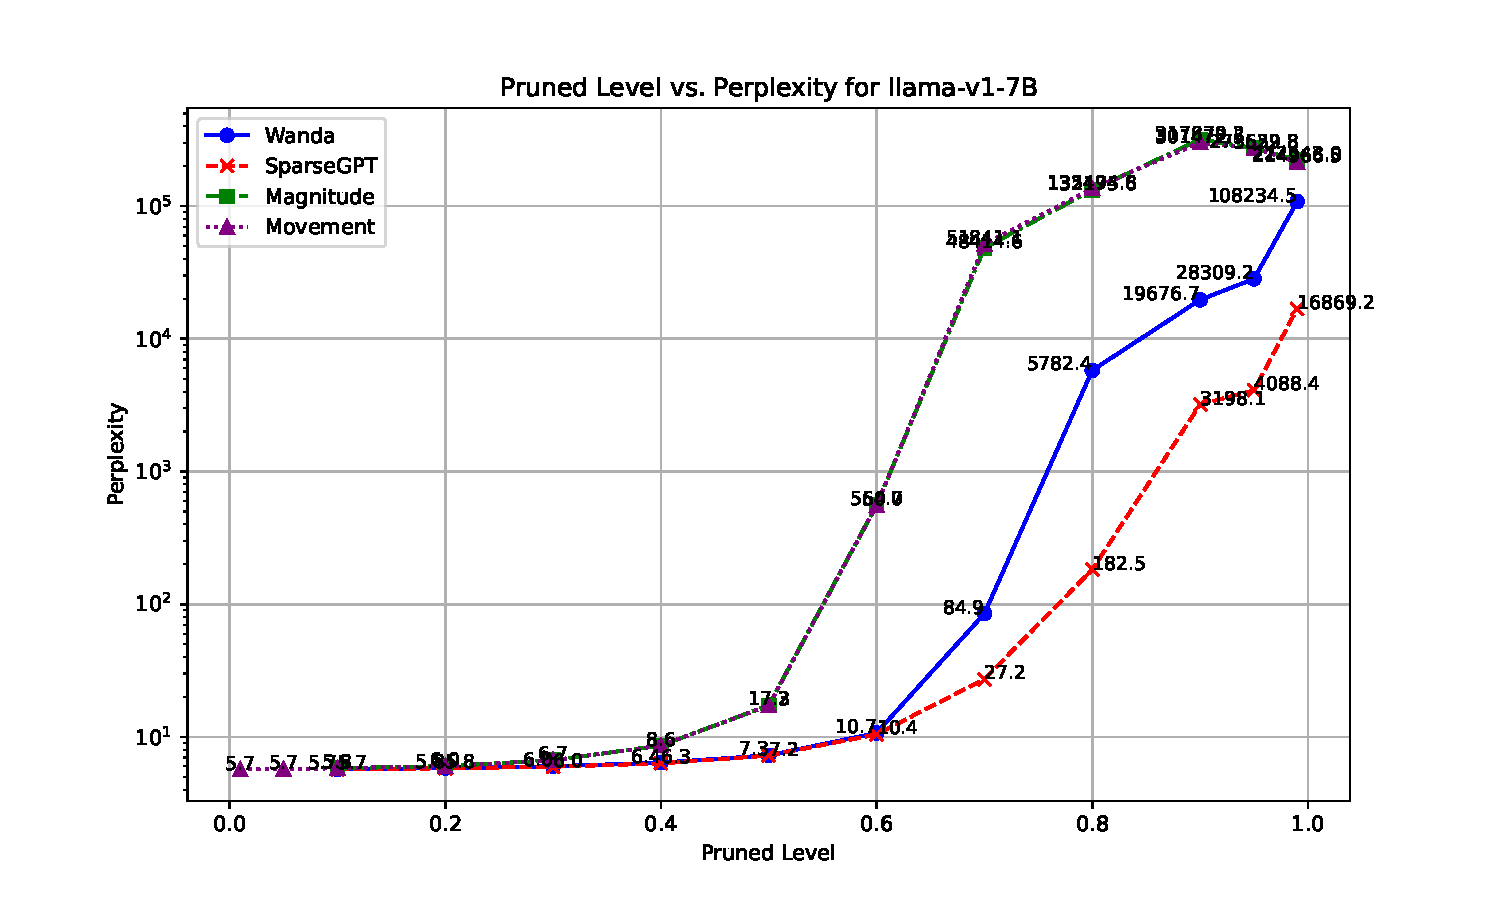
\includegraphics[width=0.8\linewidth]{fig1.pdf}
\end{center}
\caption{Pruned Level vs. Perplexity for llama-v1-7B}
\label{fig:human}
\end{figure}

\begin{figure}[h]
\begin{center}
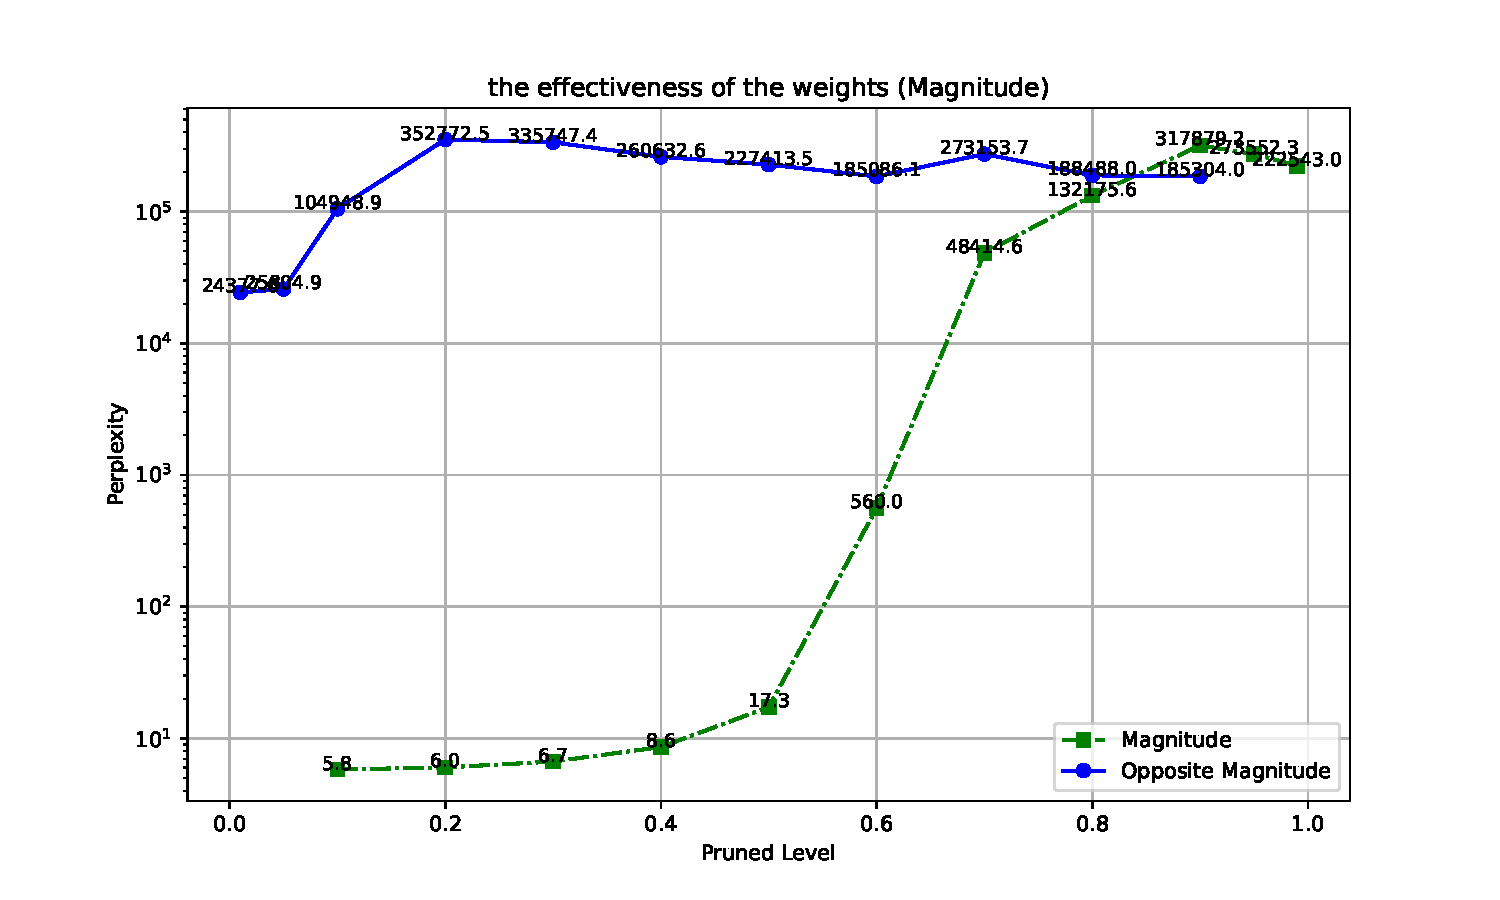
\includegraphics[width=0.8\linewidth]{fig2.pdf}
\end{center}
\caption{Effectiveness of the weights indicator}
\label{fig:weights}
\end{figure}

\begin{figure}[h]
\begin{center}
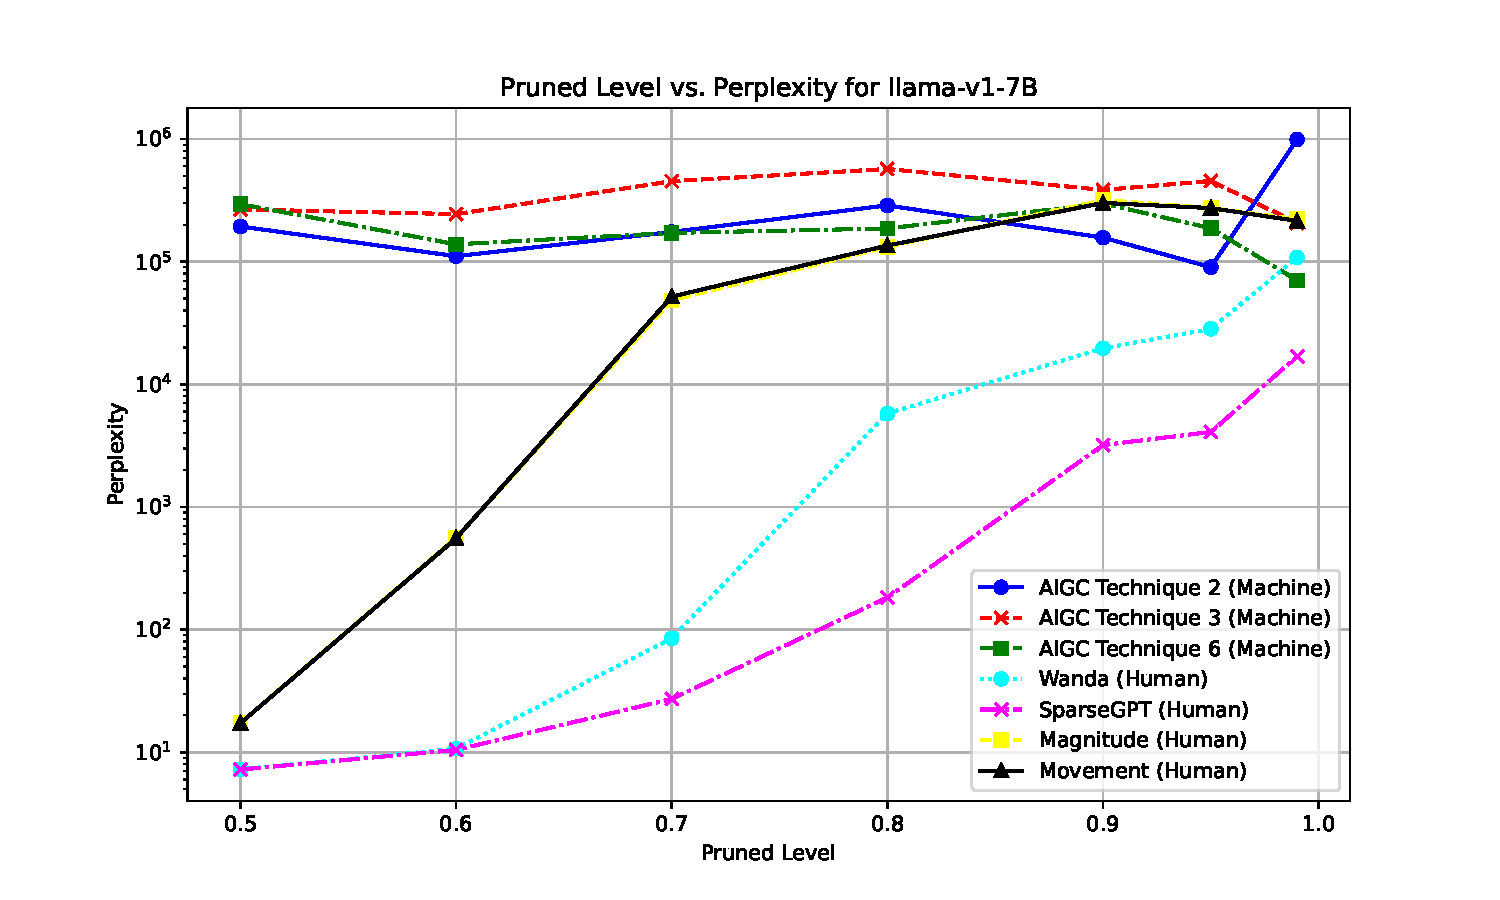
\includegraphics[width=0.8\linewidth]{fig3.pdf}
\end{center}
\caption{Performance Evaluation between Machine \& Human}
\label{fig:humanandmachine}
\end{figure}

\section{Conclusion}
\label{conclue}

In this paper, we have introduced several novel algorithms for model pruning in large language models and large vision models. Through comparison with query wheel and query covering approaches, our methodology, which attempts to estimate the likelihood of neurons resulting in expected results based on diverse neuron features, collections, and query statistics, has demonstrated significant improvement over prior work as evidenced by our experimental results. For future work, we plan several extensions. This includes conducting experiments with other language models that may potentially achieve even better pruning performances. We also aim to optimize our approach further, such as exploring hybrid methods.

Additionally, we plan to study the tradeoff between model size and query cost under different cost models and for actual query processing algorithms. This research holds promise for enhancing the efficiency and performance of large language and vision models through more effective pruning techniques.

\section{Acknowledgments}
This research was supported by a grant from *.

\bibliography{iclr2025_conference}
\bibliographystyle{iclr2025_conference}

\appendix
\section{Vision Models}

\section{MAMA on previous models}

\section{Additioanl Baselines}

\section{COMPLEMENTARY EXPERIMENTAL RESULTS}

\end{document}